\section{Our Approach: Classification and Active Learning}
\label{sec:classifierlearning}
In this section, we present details on how candidate loop invariants are generated. Algorithm~\ref{classification} shows how $actL(SP)$ is implemented in general, i.e., it iteratively generates a candidate through classification (at line 3) and improves it through active learning (at line 5) until a fixed point is reached. Note that any time a counterexample is identified (at line 2), our approach exits and reports that the Hoare triple is disproved.

\begin{algorithm}[t]
\SetAlgoVlined
\Indm
\Indp
\While{true} {
    if ($CE(SP)$ is not empty) { exit and report ``disproved''; } \\
    let $\phi$ be a set of candidates generated by $classify(SP)$\;
%    let $c$ be $classify(Positive(SP), Negative(SP))$\;
%    //alternatively: let $c$ be $classify(Positive(SP), Negative(SP) \cup NP(SP))$; \\
%    //alternatively: let $c$ be $classify(Positive(SP) \cup NP(SP), Negative(SP))$; \\
    if ($\phi$ is the same as last iteration){ return $\phi$; } \\
    add $selectiveSampling(\phi)$ into $SP$\;
    add all valuations $s'$ such that $s \Rightarrow s'$ for some $s \in SP$ into SP\;
}
\caption{Algorithm $actL(SP)$}
\label{classification}
\end{algorithm}

The method call $classify(SP)$ at line 3 in Algorithm~\ref{classification} generates a candidate invariant based in classification. Intuitively, since we know that valuations in $Positive(SP)$ must satisfy $Inv$ and valuations in $Negative(SP)$ must not satisfy $Inv$, a predicate separating the two sets (a.k.a.~a classifier) may be a candidate invariant. In the following, we fix two disjoint sets of samples $P$ and $N$ and discuss how to automatically generate classifiers separating $P$ and $N$. For now, $P$ can be understood as $Positive(SP)$ and $N$ can be understood as $Negative(SP)$. We discuss alternatives in Section~\ref{alternative}.

\subsection{Linear and Polynomial Classifiers}
To automatically generate classifiers separating $P$ and $N$, we apply existing classification techniques. There are many classification algorithms, e.g., perceptron~\cite{perceptron}, decision tree~\cite{quinlan1986induction}, Support Vector Machine (SVM)~\cite{svm:original} and neutral network~\cite{nn}.
In our approach, the classification algorithms must generate perfect classifiers. Formally, a perfect classifier $\phi$ for $P$ and $N$ is a predicate such that $s \in \phi$ for all $s \in P$ and $s \not \in \phi$ for all $s \in Negative$. Furthermore, the classification algorithms must generate classifiers which are human-interpretable or can be handled by existing program verification techniques.
In the following, we show how to adopt previously proposed algorithms~\cite{sharma2012interpolants} to generate classifiers based on SVM. Next, we extend the algorithms to generate disjunctive invariants. Lastly, we show how to improve all these candidates systematically through active learning.

In~\cite{sharma2012interpolants}, the authors propose to use SVM to generate candidate invariants. SVM is a supervised machine learning algorithm for classification and regression analysis~\cite{svm:original}.
In general, the binary classification functionality of linear SVM works as follows. Given two sets of samples $P$ and $N$, SVM generates a perfect classifier to separate them if there is any.
In the following, we write $svm(P, N)$ to denote the function which returns a perfect linear classifier for $P$ and $N$ if there is any; or returns $\textsc{null}$ otherwise. We refer the readers to~\cite{svm:smo} for details on how the classifier is computed. In this work, we always choose the \textit{optimal margin classifier} if possible. Intuitively, the optimal margin classifier could be seen as the strongest witness why $P$ and $N$ are different.
SVM by default learns classifiers in the form of a linear inequality (a.k.a.~a half space), e.g., in the form of $a x + b y \geq c$ where $x$ and $y$ are variables whereas $a$, $b$, and $c$ are constants.

In practice, linear classifiers may not be sufficient and thus more expressive invariants are necessary. We can extend SVM to learn polynomial classifiers. Given two sets of samples $P$ and $N$ as well as a degree of the polynomial classifier, we can systematically map all the samples in $P$ (similarly $N$) to a set of samples $P'$ (similarly $N'$) in a high dimensional space. For instance, assume that the target degree be 2, the sample valuation $\{ x \mapsto 2, y \mapsto 1\}$ in $P$ is mapped to $\{x \mapsto 2, y \mapsto 1, x^2 \mapsto 4, xy \mapsto 2, y^2 \mapsto 1\}$.
SVM is then applied to learn a perfect linear classifier for $P'$ and $N'$. Mathematically, a linear classifier in the high dimensional space is the same as a polynomial classifier in the original space~\cite{svm:kernel}.
We remark that the size of each sample in $P'$ or $N'$ grows rapidly with the increase of the degree and thus the above method is often limited to polynomial classifiers with relatively low degree.

A polynomial classifier can represent classifiers in the form of disjunctive or conjunctive linear inequalities. For instance, the classifier $(x \ge d_0) \wedge (x \le d_1)\big) \vee (x \ge d_2)$
where $d_0 < d_1 < d_2$ are constants can be represented as follows.
\[
x^3 + (d_0d_1 + d_0d_2 + d_1d_2)x^2 - (d_0 + d_1 + d_2)x - d_0d_1d_2 \geq 0
\]
However, it is not always possible, i.e., some conjunctive or disjunctive linear inequalities cannot be expressed in the form of a polynomial classifier. One such simple example is: $x \ge 0 \land y \ge 0$.

In~\cite{sharma2012interpolants}, an algorithm for learning conjunctive classifiers is proposed. The idea is to pick one sample $s$ from $N$ each time and identify a classifier $\phi_i$ (i.e., a linear or polynomial one) to
separate $P$ and $\{s\}$, remove all samples from $N$ which can be correctly classified by $\phi_i$, and then repeat the process until $N$ becomes empty. The conjunction of all the classifier is then a perfect classifier. We refer the readers to~\cite{sharma2012interpolants} for details of the algorithm. %This approach however may learn a classifier with many clauses. In the worse case, if each classifier $\phi_i$ only classifies the one sample $s$, the returned classifier would conjunct as many clauses as the number of samples in $N$.

\subsection{Disjunctive Classifiers}
It is known~\cite{DBLP:conf/cav/SharmaDDA11,DBLP:conf/pldi/GulwaniSV08} that it is challenging to automatically generate disjunctive invariants, whereas certain loops can only be proved with disjunctive invariants. In the following, we show how to learn disjunctive invariants through classification. Our observation is that a disjunctive invariant is needed often when the loop contains multiple branches. For instance, proving the Hoare triple shown on the left of Figure~\ref{fig:disjunctive:example} requires the loop invariant $x > 0 \lor y > 0$, which is due to the conditional branch at line 3; and the Hoare triple shown on the right of Figure~\ref{fig:disjunctive:example} (adopted from~\cite{DBLP:conf/popl/HenzingerJMS02}) can be proved with the loop invariant: $lock = 0 \lor new = old$. The reason that such a loop invariant is required is due to the conditional branch at line 5. Based on this observation, we apply the following approach to learn conjunctive or disjunctive invariants.

Assume that the loop body $Body$ contains a finite set of control locations. For instance, the loop in the first program in Figure~\ref{fig:disjunctive:example} has two locations: line 3 and 4. Given a valuation of $V$, say $s$, we write $visit(s)$ to be the set of control location which is visited if we execute the program with initial variable valuation $s$ during the first iteration of the loop. For instance, given the second program in Figure~\ref{fig:disjunctive:example}, $visit(\{lock \mapsto 0, new \mapsto 0, old \mapsto 1\})$ returns $\{\}$. We first partition $P$ into a set of disjoint partitions such that all valuations in the same partition $P_i$ visits the same set of control locations. Next, we apply the above-mentioned classification algorithms to learn a classifier for each partition, i.e., we learn a classifier $\phi_i$ for partition $i$ separating $P_i$ from $N$.
Since any sample in $P_i$ satisfies $\phi_i$ and any sample in $N$ does not satisfies, the disjunction $\bigwedge_i \phi_i$ is then a perfect classifier separating $P$ from $N$.

\begin{example}
Given the program shown on the left of
\end{example}

%\begin{figure}[t]
%   \begin{subfigure}{0.5\textwidth}
%    \raggedright
%    % \vspace{0.5cm}
%    \[
%      \begin{array}{ll}
%      1 & \code{assume(x~{>}~0~ {||} ~y~{>}~0);}  \\
%      2 & \code{while(x~{+}~y~{\le}-2)\{}  \\
%      3 & \code{\quad if~(x~{>}~0) ~~~x{++};}  \\
%      4 & \code{\quad else~ ~~~y{++};}\\
%      5 & \code{\}} \\
%      6 & \code{assert(x~{>}~0~ {||} ~y~{>}~0);}\\
%      \end{array}
%    \]
%%     \caption{A sample program}
%%     \label{fig:sl1:example:program}
%   \end{subfigure}%
%   \begin{subfigure}{0.5\textwidth}
%      \[
%      \begin{array}{ll}
%      1 & \code{assume(x < 0)} \\
%      2 & \code{while(x < 0)\{}  \\
%      3 & \code{~~~ \quad x = x + y;}  \\
%      4 & \code{~~~ \quad y++; \}}  \\
%      5 & \code{\}} \\
%      6 & \code{assert(y>0);}
%      \end{array}
%    \]
%   \end{subfigure}
%\caption{Sample programs with disjunctive loop invariants}
%\label{fig:disjunctive:example}
%\end{figure}

%\subsubsection{Disjunctive Invariants for Loop Body with 2 Branches}
%Formally, the Hoare triple for any loop body with two branches can be expressed in the following form on the left side.
%% where $\mathit{Pre}$ is named the precondition while $\mathit{Post}$ is named the postcondition, and $\mathit{Cond}$ is named the loop condition.
%In the loop body, $\mathit{C_1}$ guards the first branch $\mathit{Body_1}$, while $\mathit{\neg C_1}$ guards the other branch $\mathit{Body_2}$.
%\begin{align}
%&\{\mathit{Pre}\} && \emph{Pre} \Rightarrow \emph{$Inv_1$} \vee \emph{$Inv_2$} \label{ext:inv:pre}\\
%&\mathit{while} (\mathit{Cond}) \{ && \\
%&~~~~~~~~\mathit{if} (\mathit{C_1}) ~~\{ \mathit{Body_1} \} && \{(\emph{$Inv_1$} \vee \emph{$Inv_2$}) \wedge Cond \wedge C_1\} Body_1 \{\emph{$Inv_1$}\} \label{ext:inv:loop:b1}\\
%&~~~~~~~~\mathit{else} ~~\{ \mathit{Body_2} \} && \{(\emph{$Inv_1$} \vee \emph{$Inv_2$}) \wedge Cond \wedge \neg C_1\} Body_2 \{\emph{$Inv_2$}\} \label{ext:inv:loop:b2}\\
%&\} && \\
%&\{\mathit{Post}\} && (\emph{$Inv_1$} \vee \emph{$Inv_2$}) \wedge \neg Cond \Rightarrow \emph{Post} \label{ext:inv:post}
%\end{align}
%If the Hoare triple is valid, $Inv_1 \vee Inv_2$ that satisfies the conditions on the right side is defined as the loop invariant for the program,
%in which $Inv_1$ and $Inv_2$ are invariants for corresponding branches.
%% For example, $Inv_1$ is the branch invariant for the first branch as it is evaluated true after execution of $Body_1$ as shown in~\ref{sl1:ext:inv:loop:b1}.
%In our context, branch invariant is a property that always holds for the given branches.
%
%% in which $Inv_1$ and $Inv_2$ are named as branch invariants for the two branches.
%%Assume the invariant for the loop is in the form of $Inv_1 \vee Inv_2$.
%%Note that, any invariant $i$ can be converted to this form by linking itself with disjunction operator, such as $i \vee i$.
%%If there are $Inv_1$ and $Inv_2$ satisfy the following conditions,
%%then $Inv_1 \vee Inv_2$ is a loop invariant for the original program.
%
%In the following, we prove that for loop programs with 2 branches,
%the above definition of loop invariant is equivalent with the previous invariant definition.
%Therefore, we need to prove such $Inv_1 \vee Inv_2$ is a valid loop invariant for the loop program,
%and any loop invariant for the program can be written as $Inv_1 \vee Inv_2$, where $Inv_1$ and $Inv_2$ are branch invariants.
%
%% \begin{theorem}
%% Algorithm~\ref{ta_feasiblefuncwithsim} is sound and complete.
%% \vspace{-1mm}
%% \end{theorem}
%% \noindent \textbf{Proof:} As we discussed the difference between Algorithm~\ref{ta_feasiblefuncwithsim} and Algorithm~\ref{ta_feasiblefunc}, given a transition system $\mathcal{L}$ with a set of initial states $Init$, the transition relation $Tr$ and a set of \buchi conditions $J$, while $IsEmpty(Init, Tr, J)$ is checking the emptiness of $\mathcal{L}$, $IsEmpty_{sim}(Init, Tr, J)$ is actually checking the emptiness of the transition system $\mathcal{L'}$. Thus, the correctness of Algorithm~\ref{ta_feasiblefuncwithsim} is obtained based on Theorem~\ref{theoremofabstractedsystem}.\hfill \qed \\
%
%\begin{theorem}
%\label{thm:disjunctive:is:invariant}
%	$Inv_1 \vee Inv_2$ is a loop invariant for the given loop program.
%\end{theorem}
%
%\noindent \textbf{Proof:} In order to prove $Inv_1 \vee Inv_2$ is a loop invariant for the program,
%we need to show it satisfies all the three conditions~\ref{org:inv:pre}, ~\ref{org:inv:loop} and ~\ref{org:inv:post}.
%
%By simply substituting $Inv$ with  $Inv_1 \vee Inv_2$,
%we can see $Inv_1 \vee Inv_2$ satisfies condition~\ref{org:inv:pre} and ~\ref{org:inv:post}.
%For condition~\ref{org:inv:loop},
%as the valuations obtained through the two branches satisfy $Inv_1$ and $Inv_2$ respectively,
%the valuations for the loop body must satisfy $Inv_1 \vee Inv_2$ naturally.
%Thus, by combining the condition~\ref{ext:inv:loop:b1} and~\ref{ext:inv:loop:b2},
%\begin{align*}
%&\{(Inv_1 \vee Inv_2) \wedge Cond \wedge C_1\} Body_1 \{Inv_1\} \\
%&\{(Inv_1 \vee Inv_2) \wedge Cond \wedge \neg C_1\} Body_2 \{Inv_2\}
%\end{align*}
%we can get $\{(Inv_1 \vee Inv_2) \wedge Cond\}~if (C1)~{Body_1}~else~{Body_2}~\{Inv_1 \vee Inv_2\}$,
%which satisfies the second condition in loop invariant definition.
%
%Therefore, $Inv_1 \vee Inv_2$ is a loop invariant for the given loop program. %\hfill \qed \\
%
%\begin{theorem}
%\label{thm:invariant:is:disjunctive}
%	Any invariant $Inv$ for the given loop program with branches can be expressed in the form of $Inv_1 \vee Inv_2$.
%\end{theorem}
%
%\noindent \textbf{Proof:} If $Inv$ is a loop invariant for the given loop program,
%then $Inv$ satisfies the three conditions ~\ref{org:inv:pre}, ~\ref{org:inv:loop} and ~\ref{org:inv:post}.
%As $Inv = Inv \vee Inv$ always holds, we assign $Inv_1 = Inv$ and $Inv_2 = Inv$.
%Then the three conditions can be easily verified. %\hfill \qed \\
%
%\subsection{Disjunctive Invariants for Loop Body with $\emph{n}$ Branches}
%For the loop body with $n$ branches and valuations for each branch satisfy $Inv_1$, $Inv_2$, $\cdots$, $Inv_n$ respectively,
%it is similar to prove the loop invariant defined as $Inv_1 \vee Inv_2 \vee \cdots \vee Inv_n$ is equivalent to the invariant defined before,
%which means we can apply same technique to combine all the branch invariants together as the candidate loop invariant.
%
%\subsubsection{Disjunctive Invariant Learning Algorithm}
%Assume a Hoare triple that there are 2 branches in the loop body is given,
%and thus our invariants can be written as $(Inv_1 \vee Inv_2 \vee \cdots \vee Inv_n)$.
%Without loss of generality, we take branch $B_i~(1 \le i \le n)$ , whose branch invariant $Inv_i$ accordingly, as an example.
%We build a new set $\mathit{Positive\_B_i}$ by extracting the valuations in $\mathit{Positive}$ which are obtained after passing branch $B_i$.
%According to definition in~\ref{ext:inv:loop:b1} and \ref{ext:inv:loop:b2},
%valuations in $\mathit{Positive\_B_i}$ must satisfy $Inv_i$.
%For any valuation $s \in \mathit{Negative}$,
%we can infer $s \not \models Inv_i$ since $s \not \models Inv_1 \vee Inv_2 \vee \cdots \vee Inv_n$.
%Therefore, all the valuation in $\mathit{Negative}$ fails any branch invariant $Inv_i $.
%
%As a result, we can apply Algorithm~\ref{alg:polynomialSVM} on set $\mathit{Positive\_B_i}$ against set $\mathit{Negative}$ to learn a classifier as the candidate for $Inv_i$.
%Similar procedures are adapted for other branches and the approach can generate an invariant candidate by combining all the classifiers.
%
%\paragraph{Example}
%In the following, we use an illustrative example to show how our framework works on disjunctive invariant learning.
%
%% can apply the primary SVM
%\begin{figure}[t]
%  % \begin{subfigure}{0.5\textwidth}
%    \raggedright
%    % \vspace{0.5cm}
%     \vspace{-0.2cm} \[
%      \begin{array}{ll}
%      1 & \code{void~foo(int ~x{,} ~int~y)\{} \\
%      2 & \code{~~~ assume(x~{>}~0~ {||} ~y~{>}~0);}  \\
%      3 & \code{~~~ while(x~{+}~y~{\le}-2)\{}  \\
%      4 & \code{~~~ \quad if~(x~{>}~0) ~~~x{++};}  \\
%      5 & \code{~~~ \quad else~ ~~~y{++};}\\
%      6 & \code{~~~\}} \\
%      7 & \code{~~~assert(x~{>}~0~ {||} ~y~{>}~0);}\\
%      8 & \}
%      \end{array}
%    \]
%  %   \vspace{-0.2cm}
%  %   \caption{A sample program}
%  %   \label{fig:sl1:example:program}
%  % \end{subfigure}%
%  % \begin{subfigure}{0.5\textwidth}
%  %   \centering
%  %   \includegraphics[scale=0.25]{figures/sl1_cfg.pdf}
%  %   \caption{The Control flow graph of the loop}
%  %   \label{fig:sl1:example:cfg}
%  % \end{subfigure}
%\caption{Disjunctive loop example}
%\label{fig:disjunctive:example}
%\end{figure}
% \vspace{-0.2cm}
%We collect and label the variable valuations at line 4 and line 5.
%After classifier learning phase, a classifier $x>0$ can be learned at line 4 while $y>0$ can be obtained at line 5.
%Thus, we can get a candidate invariant $(x>0) \vee (y>0)$ by combining the classifiers together.
%Apparently, $(x>0) \vee (y>0)$ is the actual invariant for the given program.

\subsection{Active Learning}
One fundamental problem on applying machine learning techniques to learn loop invariants is the we often have only a limited set of samples, i.e., with the limited samples in $Positive(SP)$ and $Negative(SP)$,
it is unlikely that we can obtain an ``accurate'' classifier. For instance, in Example~\ref{example2}, $Positive(SP)$ is $\{(1, 2),(11, 5)\}$ and $Negative(SP)$ is $\{(100, 0)\}$. A linear classifier identified using SVM is: $3x-10y \leq 152$. Although this classifier perfectly separates the two sets, it is not useful in proving the Hoare triple and is clearly the result of having limited samples.
One obvious way to overcome this problem is to generate more samples. However, often a large number of samples are necessary in order to learn the correct classifier. One particular reason is that we often need the samples right on the classification boundary in order to learn the correct classifier, which are often difficult to obtain through random sampling. In existing guess-and-check approaches~\cite{sharma2012interpolants,sharma2013verification,DBLP:conf/esop/0001GHALN13,sharma2014invariant}, the problem is overcome by checking whether candidate invariants proves the Hoare triple through program verification. So that the invariant can be refined with new samples which are provided as counterexamples by the program verification engine. The issue is that often many iterations of guess-and-check are required so that the invariant would converge to the correct one.

Researchers in the machine learning community have studied extensively on how to overcome the problem of limited samples and one of the remedies is active learning~\cite{DBLP:series/synthesis/2012Settles}.
Active learning is proposed in contrast to passive learning. A passive learner learns from a given set of samples which it has no control, whereas an active learner actively selects what samples to learn from. It has been shown that an active learner can sometimes achieve good performance using far less samples than would otherwise be required by a passive learner~\cite{DBLP:conf/mm/TongC01,DBLP:journals/jmlr/TongK01}. Active learning can be applied for classification or regression. In this work, we apply it for improving the candidate assertions generated by the above-discussed classification algorithms.

A number of different active learning strategies on how to select the samples to learn from have been proposed. For instance, version space partitioning~\cite{DBLP:conf/icml/RuffD89} tries to select feature vectors on which there is maximal disagreement between classifiers in the current version space (e.g., the space of all classifiers which are consistent with the given data); uncertainty sampling~\cite{DBLP:conf/sigir/LewisG94} maintains an explicit model of uncertainty and selects the vector that it is least confident about. The effectiveness of these strategies can be measured in terms of the labeling cost, i.e., the number of labeled samples needed in order to learn a classifier which has a classification error bounded by some threshold $\epsilon$. For some classification algorithms, it has been shown that active learning reduces the labeling cost from $\Omega(\frac{1}{\epsilon})$ to the optimal $O(d\lg\frac{1}{\epsilon})$ where $d$ is the dimension of feature vectors~\cite{DBLP:conf/nips/Gilad-BachrachNT05,DBLP:conf/nips/Dasgupta05}. That is, if passive learning requires a million samples, active learning may require just $\lg 1000000$ ($\approx 20$) to achieve the same accuracy.

In this work, we adopt the active learning strategy for SVM proposed in~\cite{DBLP:conf/icml/SchohnC00}, called selective sampling, which has been shown to be effective in achieving a high accuracy with fewer examples in different applications~\cite{DBLP:conf/mm/TongC01,DBLP:journals/jmlr/TongK01}. In particular,
at line 5 of Algorithm~\ref{classification}, after obtaining a classifier $\phi$ based on existing samples in $SP$, we apply method $selectivesampling(\phi)$ to selectively generate new samples, which works by generating samples on (or nearby) the current classification boundary $\phi$. ,
Afterwards, the samples are added into $SP$ at line 5 and 6 and we repeat from line 2  until the classifier converges.
%For instance, Figure~\ref{fig:running:example:sampling} shows where the set of valuations
%in $\mathit{Positive}$, $\mathit{Negative}$ and $\mathit{NP}$ locate geographically in a 2-D plane for our running example.
%In particular, valuations in $\mathit{Positive}$ are labeled with $+$; % and color green;
%valuations in $\mathit{Negative}$ are labeled with $-$; % and color red;
%and valuations in $\mathit{NP}$ are labeled with ?. % and color yellow.
%And there are three areas: a pure positive area with color green, a pure negative area with color red, and a mixed area with color yellow.
%The mixed area exists because our labeling method depends much on the observed program valuation sequences.
%

For classifiers in the form of linear inequalities, identifying samples on or nearby the classification boundary is straightforward. In the above example, given the current classifier $3x-10y \leq 152$, we apply selective sampling and generate new valuations $\{x \mapsto 7, y \mapsto 13\}$ and $\{x \mapsto 14, y \mapsto -11\}$ by solving the equation $3x-10y = 152$. For classifiers in the form of polynomial inequalities, the problem is slightly more complicated since existing equation system solvers for multi-variable polynomial equations has limited scalability. We thus adopt a simple approach, which we illustrate through a simple example in the following. Assume that we learn a polynomial classifier: $-4x^2+2y \geq -11$. The following steps are applied to identify samples right on the classification boundary.
\begin{enumerate}
\item Choose a variable in the classifier, e.g., $x$.
\item Generates random value for other variables. For example, we let $y$ be $12$.
\item Solve the equation $-4x^2+2y = -11$ after substituting variables with their values. If there is no solution, go back to (1) and retry.
In our example, $x \approx 2.9580$.
%\item Add a random variance $\epsilon \in [-1, 1]$ to the value of the picked variable. Here we add $\epsilon = 0.4$ to the value of $x$, and thus the new value of $x$ is $3.3580$.
\item Roundoff the values of all the variables according to their types in the program. In our example, we obtain the valuation $\{x \mapsto 3, y \mapsto 12\}$.
\end{enumerate}
In the case that a conjunctive or disjunctive classifier (of linear or polynomial inequalities) is learned, we apply the above approach to each and every clause in the classifier to obtain new samples. With the help of active learning and selective sampling, we can often reduce the number of learn-and-check iterations. As we show in Section~\ref{sec:evaluations}, with active learning, often one iteration of learn-and-check is sufficient to prove the Hoare triple.

\paragraph{Selective sampling vs. other sampling} In this work, we collect samples in three different ways: \emph{random sampling}, \emph{selective sampling} based on active learning and \emph{sampling through verification}.
Random sampling provides us the initial set of samples. The cost of generating a random sample is often low. However we often need a huge number of random samples in order to learn accurately. Selective sampling bares a slightly higher cost since often it requires to solve some equation system. However, it has been shown that selective sampling is often beneficial compared to random sampling~\cite{DBLP:conf/mm/TongC01,DBLP:journals/jmlr/TongK01}. The last sampling is sampling through verification. When a candidate invariant fails any of the three conditions (1), (2) and (3) in the candidate verification stage, the verifier could provide counter-examples, which are added as new samples. Sampling through verification provides useful new samples by paying a high cost. Thus, in this work, our approach is to start with random sampling, use selective sampling to improve the classifier as much as possible and apply sampling through verification only as the last resort.

Figure~\ref{fig:sampling} visualizes how different sampling methods are related to each other in a 2-D plane. We start with the figure in the top-left corner.
The (green) area above the line represents the space covered by the actual invariant. The dots are the samples obtained through random sampling.
Based on these samples, a classifier is learnt to separate the random samples, as shown in the top-right figure.
With this learnt invariant, selective sampling would us to identify those samples on the classification boundary based on the learnt classifier, as shown in the bottom-left figure.
In comparison, sampling through verification would provide us the sample between the two lines shown in the bottom-left figure.
It is obvious that the classifier will be improved with either selective sampling or sampling through verification, as shown in the bottom-right figure.
The benefit of always applying selective sampling before applying sampling through verification is that verification is often more costly and thus we would like to avoid it as much as possible. \\

\begin{figure}[t]
        \centering
        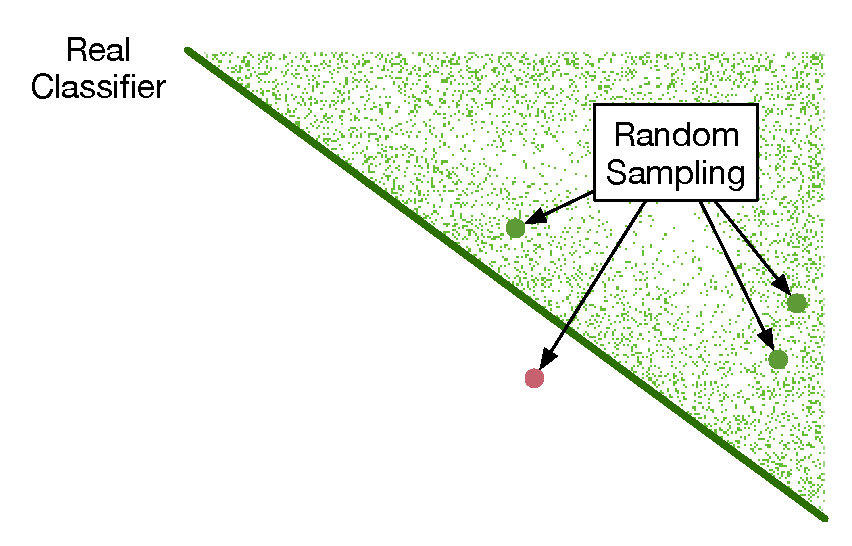
\includegraphics[scale=0.3]{figures/general-sampling-0.pdf}
%        \caption{Random Sampling}
        \centering
        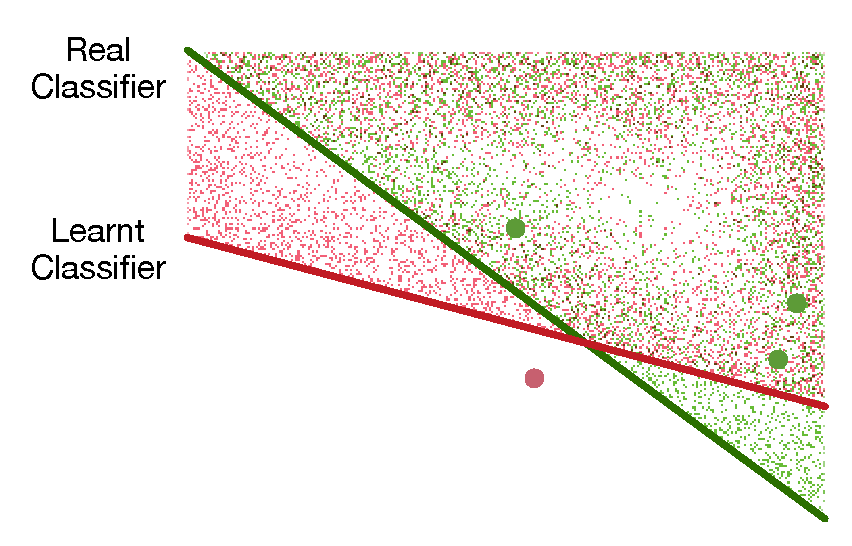
\includegraphics[scale=0.3]{figures/general-sampling-1.pdf} \\
%        \caption{Learnt Invariant}
        \centering
        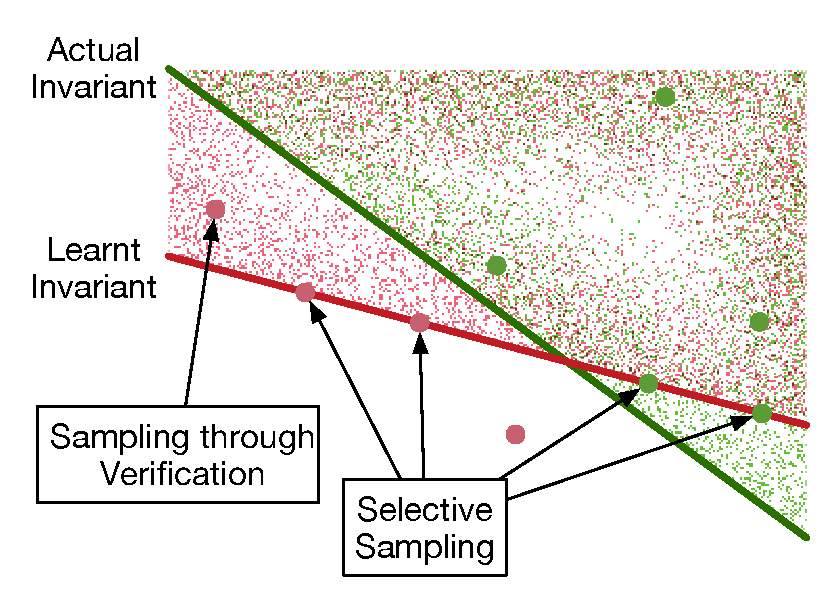
\includegraphics[scale=0.3]{figures/general-sampling-2.pdf}
%        \caption{Selective and Counter-Example Sampling}
        \centering
        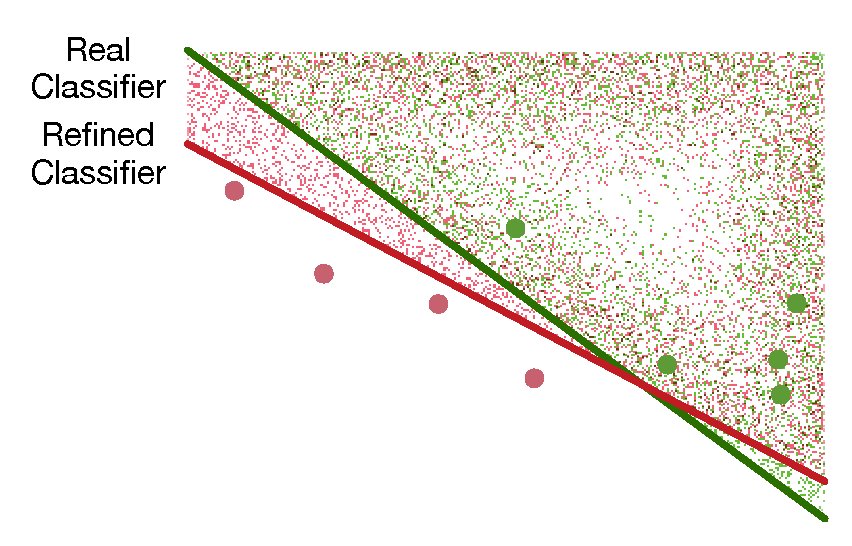
\includegraphics[scale=0.3]{figures/general-sampling-3.pdf}
%        \caption{Refined Invariant}
    \caption{Sampling approaches}
    \label{fig:sampling}
\end{figure}


\subsection{Making Use of Undetermined Samples} \label{alternative}
So far we have focused on learning and refining classifiers between $Positive(SP)$ and $Negative(SP)$. The question is then: how do we handle those valuations in $NP(SP)$, which may or may not satisfy $Inv$? If we simply ignore them, there may be a gap between $Positive(SP)$ and $Negative(SP)$ and as a result, the learnt classifier may not converge to the invariant we want, even with the help of active learning.
This is illustrated in Figure~\ref{fig:running:example:sampling}, where the set of valuations in $Positive(SP)$ (marked with $+$), $Negative(SP)$ (marked with $-$) and $NP(SP)$ (marked with $?$) for the example in Figure~\ref{fig:running:example:program} are plotted in a 2-D plane. Many samples between the line $x=y$ and $x-y=16$ may be contained in $NP(SP)$. As a result, without considering the samples in $NP(SP)$, classifiers located in the $NP(SP)$ region (e.g., $x - y \leq 10$, or $x - y \leq 13$) may be learned to perfectly classify $Positive(SP)$ and $Negative(SP)$. Worse, identifying more samples may not help to improve the classifier if the new samples are in $NP(SP)$ or are already classified by the existing classifier.

To overcome the problem, in addition to learn a classifier separating $Positive(SP)$ and $Negative(SP)$, we learn candidate invariants making use of $NP(SP)$, i.e., classifiers separating $Positive(SP)$ from $Negative(SP) \cup NP(SP)$ (i.e., assuming valuations in $NP(SP)$ fail the actual invariant), and classifiers separating $Negative(SP)$ from $Positive(SP) \cup NP(SP)$ (i.e., assuming valuations in $NP$ satisfy the actual invariant).
We remark that active learning is applied to all these candidates until they converge. For the example in Figure~\ref{fig:running:example:program}, if we focus classifiers in the form of linear inequalities, the classifier separating $Positive(SP)$ from the rest converges to $\textsc{null}$ (no such classifier), whereas the classifier separating $Negative(SP)$ from the rest converges to $x - y \leq 16$, which can be used to prove the Hoare triple.

\begin{figure}[t]
      \centering
      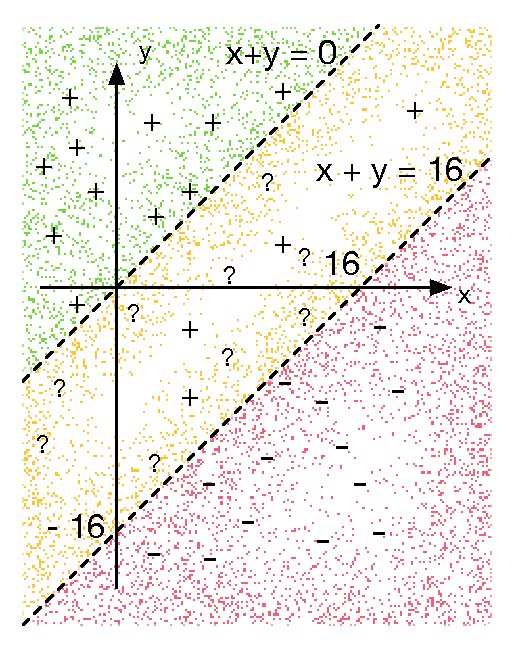
\includegraphics[scale=0.42]{figures/running-sampling.pdf}
      \caption{Distribution of samples}
      \label{fig:running:example:sampling}
\end{figure}
